%!TeX spellcheck = en-US
\documentclass[../main.tex]{subfiles}
\begin{document}
\chapter{Scenario}
\label{chap:avionicsprot}

The technological explosion of the last years influenced also the aviation sector. Better planning, more efficient aircrafts and many other management improvements brought the price of airline tickets down making traveling by plane accessible to anyone. More recently the drone market rapidly grew to the point where every professional and amateur video maker must have at least one drone to capture great aerial shots that in the past could only be done by using helicopters. Moreover companies like \textit{Amazon} and \textit{DHL} successfully tested a parcel delivery service operated by drones~\cite{primeair} while other companies like \textit{Facebook} and \textit{Google} started testing an affordable and reliable method to bring internet connection to remote areas of the planet~\cite{loon}. Furthermore, companies like PrecisionHawk~\cite{prechwk} developed accurate sensors to be used with different drones that allow the user to perform many different measurements. \acrlong{uav}s (\textbf{\acrshort{uav}}) are spreading also in the 4.0 agriculture, \acrlong{sar} (\textbf{\acrshort{sar}}) and general emergency fields\cite{vvff}. Nowadays Military operations are more and more drone-centered, therefore armed forces, from infantry to flying squadrons, are equipped with different kinds of \textbf{\acrshort{uav}}. All this sudden progress has led to overcrowded skies in which the innovation in the \acrlong{atm} (\textbf{\acrshort{atm}}) field must be continuously updated. New systems have been built with a strong push of implementing \acrshort{iot} paradigm in respect with the \textbf{\acrshort{atm}}, \textbf{\acrshort{uav}} and avionics systems.

Airplanes can no longer be seen as the main users of the sky. A wider spectrum of flying objects should be considered given the different nature of their functions. Aircrafts are divided into different categories depending on the maximum altitude, their weight and other parameters. Commercial drones, such as \textit{Amazon} or cinematography ones are now developing capabilities similar to small aircrafts in terms of performance. Similarly \textit{Facebook} Aquila drones have the same wingspan as a Boeing 737 and they can fly at a considerably high altitude\cite{fbaquila}. Also Project Loon internet balloons (\textit{Google}) travel at high altitude and through busy airspace. In addition, there are many other objects like gas balloons, helicopters and gliders operating in specific areas and airspace class that must be tracked, managed and monitored efficiently to ensure high safety standards.

The development of a new technology brings a lot of challenges, some of them in the cybersecurity realm.
In particular, Costin and Francillon~\cite{costin2012ghost} demonstrated in 2012 that it is easy and cheap to perform various operational attacks on ADS-B protocols in particular, and \textbf{\acrshort{atm}} and \textbf{\acrshort{atc}} systems in general.
Subsequently, various weaknesses were demonstrated in various Air Traffic Control (ATC) protocols~\cite{renderman,teso} and avionics sub-systems.
%? ~\cite{sindragon}.
More recently, in November 2017 the news broke that back in September 2016 a team from Department of Homeland Security (DHS) was able to hack a Boeing 757 parked at the airport. The hack was described as \emph{``remote, non-cooperative, penetration''}~\cite{news-boeinghack-cso}.
Though the details were scarce because of the classified label, it was acknowledged that the team, consisting of industry experts and academics, accomplished the hack by accessing the aircraft communication systems through radio frequency communications.

Aiming at more security and in order to overcome some limitations of the old generation protocols like the absence of radar coverage in certain areas of the planet (e.g. over the ocean), a modernization of the radar and communication system was launched starting from the 80s up to the present days with the development of two generations of protocols. Standards and guidance documents for aeronautics are defined by different cooperative organizations, the major of which are \acrlong{rtca} (\textbf{\acrshort{rtca}}) in the United States, \acrlong{eurocae} (\textbf{\acrshort{eurocae}}) in Europe and \acrlong{icao} (\textbf{\acrshort{icao}}) which is a UN organization. The above mentioned organizations are non governative therefore they produce standards, guidelines or rules that will have to be adopted by the \acrlong{faa} (\textbf{\acrshort{faa}}) in the united states, by the \textbf{EUROCONTROL}\footnote{The organization that provides unique centralized platform for civil and military aviation coordination in Europe.} and the single national aviation authority of the various European countries (\textit{\acrshort{enac}/\acrshort{enav}} in Italy). This fragmentation of the establishment, the absence of a globally shared guidance on the standardization of the aviation sector (which is partially an \acrshort{icao} task.\footnote{Art 1. The contracting States recognize that every  State has complete and exclusive sovereignty over the airspace above its territory.\cite{icao7300}}) and the development of different standards to accomplish the same task have created an unclear situation about standards and regulations. NextGen has shown problems in the definition of a globally accepted family of protocols as it can be seen in the relevant section.

Aircrafts can be tracked either by a \textbf{cooperative} way  and a \textbf{non-cooperative} one:

\begin{itemize}

  \item The classic radar (or Primary Radar), based on electromagnetic waves is able to give information only on the position of an object in the sky. Such system gives a real-time image of the portion of sky it is observing, including aircrafts, birds, clouds, and any other object in its visual range making it a basic and fairly unreliable system. Since this method requires no interaction with the aircraft that is being tracked, it is called \textbf{non-cooperative} system.
  \item \acrlong{ssr} (\textbf{\acrshort{ssr}}) is an evolution of the above system. In addition to the spatial position of the aircraft, it gives further information depending on its mode of operation. This system requires an active cooperation from the aircraft which must reply to the interrogations received making it a \textbf{cooperative} system.

\end{itemize}

The cooperative systems allow to have a bidirectional data flow between aircraft and ground as well as aircraft and aircraft. This system stems from the military \acrlong{iff} (\textbf{\acrshort{iff}}) one which was developed during the Second World War. The actual civil system uses a 4 digit code called "Transponder Code" or \textbf{"Squawk"} to identify the aircraft. This communicates via a \textbf{transponder} which handles the incoming interrogations and the responses. In Figure \ref{fig:allgen} is an overview of all the protocols and their division between the old generation and the new one which is still in deployment.

\begin{figure}[htp]
  \centering
  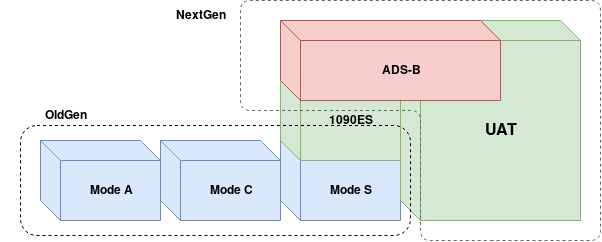
\includegraphics[scale=0.6]{images/allgen.png}
  \caption{All generation of avionics protocols}
  \label{fig:allgen}
\end{figure}

Having a continuous data flow between the aircraft and the ground is beneficial not only for the \acrshort{atm}/\acrshort{atc} but also for the airline. As a matter of fact:
\begin{itemize}
  \item Flight controllers can obtain much more information about a single aircraft, his intentions and the status of the flight. Moreover satellite based ADS-B allow to trace planes in areas where no radar coverage is available.
  \item The airline can keep track of its fleet in real time thus allowing a better planning of the turnover and, if needed, quick deployment of a substitute airplane.
  \item The maintenance branch of the airline can track in real time any anomalies reported by the instruments and sensors performing a remote analysis which will help pilots make better decisions in the troubleshooting process.
\end{itemize}

As previously mentioned the current avionics protocols can be divided in two families: \textbf{OldGen} and \textbf{NextGen}. The \textbf{OldGen} is currently deployed and used globally while the \textbf{NextGen} is standardized and set to be fully deployed by 2020. For this reason, to comply with regulations and to enhance safety Project Loon balloons are equipped with both OldGen and NextGen hardware\cite{loonadsb} while some DJI drones are compatible with NextGen protocols\cite{dji}.

In addition to their use in aircrafts both OldGen and NextGen protocols are now integrated in a big network of IoT sensors. It is currently estimated there are no less than $\countadsbrecvtotal$ air-traffic sensors/receivers integrated into crowd-sourced projects, in particular about $\countadsbrecvfradar$ in FlightRadar24~\cite{countFRadar}, around $\countadsbrecvfaware$ in Flightaware~\cite{countFAware}, and at least $\countadsbrecvopensky$ in OpenSky-Network~\cite{schafer2017opensky}. These sensors/receivers can be either general purpose devices such as RaspberryPi (RPi) and routers plugged with USB RTL-SDR dongles, or can be special-purpose ADS-B receivers using specialized FPGA implementations.
%
Moreover, it is expected the number of aircraft, including air carrier and \acrlong{ga} (\acrshort{ga}), that are equipped or upgraded with avionics embedded devices supporting ADS-B and other NextGen protocols will surpass $\countadsbrecvfaa$~\cite{countFAA}.
These numbers do not account for the considerable number of devices that are deployed at various \acrshort{atc} towers and that process avionics RF protocols. Therefore, given the number and the Critical Infrastructure (CI) functions of those devices, it is important to secure those systems and to be sure that no flaws exist in the protocols.

\section{OldGen}

The first generation of protocols is fairly simple; it uses the 1030MHz frequency for interrogation and the 1090MHz frequency for replies.
The first two protocols are \textbf{Mode A} and \textbf{Mode C}.

\textbf{Mode A} is the simplest because it responds to an interrogation request just by broadcasting the \textbf{squawk} code which was previously assigned to the pilot by the controller. In this way the controller can identify the aircraft on his screen by such code. In addition to this, the pilot can manually generate a special response called \textit{"Ident"} or \textit{"\acrshort{spi}"} (\acrlong{spi}) which is used to highlight the aircraft on the controller screen.

\textbf{Mode C} is an extension of the previous protocol which, in addition to the transponder code, sends information about the altitude and the pressure. This kind of transponders are often referred to as \textbf{Mode A/C}.

\textbf{Mode S} is the newest protocol of this family and it is an hybrid between the two generations. It was born as part of the OldGen family but at the same time it is also part of the NextGen as it can be seen in Figure \ref{fig:allgen}. As clearly explained further in the text \textbf{Mode S} in the years has undergone various enhancements and refinements in order to be used as an easy-to-deploy and affordable NextGen protocol. \textbf{Mode S} ground stations and transponders support both all call interrogations and selective interrogations, in particular each aircraft is identified by a unique 24-bit address which is part of the aircraft registration documents and should never be changed. The address is transmitted with every \textbf{Mode S} reply, which allows a \acrshort{ssr} station to perform an all call interrogation in order to acquire the address of each aircraft which can then be used to selectively interrogate them. Each ground station is identified by a 4-bit\footnote{For aircraft complying with ICAO Annex 10, Volume IV Amendment 73 a 6-bits code can be used} \acrlong{ic} (\acrshort{ic}). In this way single aircraft interrogation as well as lock-out of the aircraft can be performed in order to avoid multiple pickups of the same aircraft by different \acrshort{ssr} stations. \textbf{Mode S} messages can be of 56 or 112 bits and they are structured as in Figure \ref{fig:modes}.

\begin{figure}[htp]
  \centering
  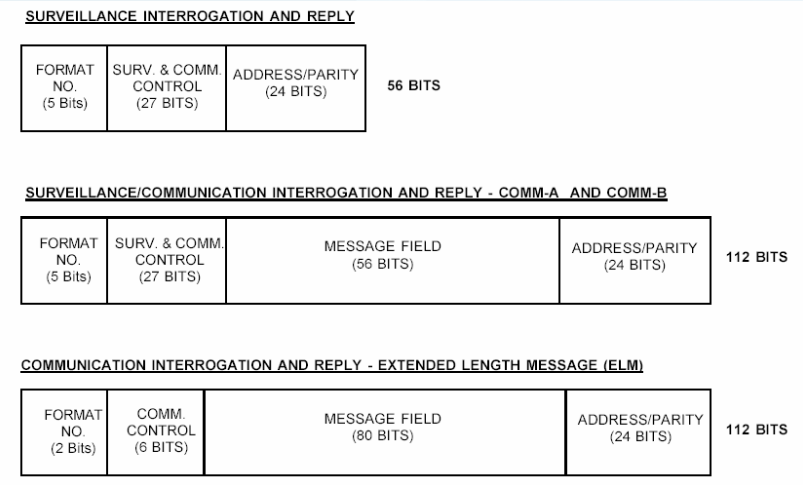
\includegraphics[scale=0.65]{images/modes.png}
  \caption{Mode S messages}
  \label{fig:modes}
\end{figure}

In \textbf{Mode S} messages the first 5 bits identify the type of message called \acrlong{df} (\acrshort{df}), then the other bits, except for the last 24, are message dependent. \textbf{Mode S} comes in two versions: \acrlong{els} (\textbf{\acrshort{els}}) and \acrlong{ehs} (\textbf{\acrshort{ehs}}). \textbf{\acrshort{els}} has been described above and is the minimum version required in European Mode S airspace. \textbf{\acrshort{ehs}} introduces some improvements:

- Reduced workload for the pilots and the controller, since some radio communications can be avoided when the controller has access to information such as the Magnetic Heading or the Selected Altitude.

- Improved Situation Awareness, since the controller can have access to a greater amount of data like Vertical Climb Rate, Magnetic Heading, Selected Altitude and similar.

- Safety Enhancements brought by data such as Selected Altitude which permits the controller to check if the aircraft is following the instructions and avoid potential collisions or level bust in advance~\cite{modesbook}.

\textbf{Mode S EHS} is a minimum requirement for some categories of aircraft flying in European Mode S airspace.

All the above protocols are at the base of the \acrlong{acas} (\textbf{\acrshort{acas}}). This system requires all flying objects to be equipped with \textbf{Mode A/C}, \textbf{Mode C} or \textbf{Mode S} transponders. In this way it can keep track of the surrounding airplanes and, in case of colliding traffic, propose vertical \acrlong{ra} (\textbf{\acrshort{ra}}). NextGen systems have enhanced \textbf{RA} capabilities. It is clear that this is a critical part of the system and, if compromised, can lead to dramatic results such as mid air collision.

\textbf{Mode A/C} and \textbf{S} are the current standards and they are widely used, notably according to the Italian regulation all aircrafts must be equipped with at least a \textbf{Mode A/C} transponder and in some particular cases with a \textbf{Mode S} transponder as it can be seen in GEN 1.5-3.1 of AIP Italia\cite{itareg}.

Beside the basic protocols described here, a more sophisticated one lays between the two generations.
The \acrlong{acars} (\textbf{\acrshort{acars}}) has been in use since 1978. At first it relied only on \acrshort{vhf} radio channels but in the years it has been improved to add other transmission means to expand coverage. It is also now deeply integrated into the aircraft systems giving it access to a large number of data and the ability to operate autonomously. Acars messages can be delivered via 3 different transmission means: \acrshort{vhf} Data Link, \acrshort{hf} Data Link and satellite. Depending on the position of the aircraft, one method can be better than the other, specifically \acrshort{vhf} works only in line of sight while satellite communication (SATCOM) is not available at the poles. \textbf{\acrshort{acars}} messages can be of 3 different types:
\begin{itemize}
  \item \acrlong{atc} messages. Used in some busy airports as an alternative to the radio. And in routes where no radio contact is possible (e.g oceanic routes).
  \item Aeronautical Operational Control (AOC) and Airline Administrative Control (AAC) used to send documents to the aircraft as well as to receive error messages or information on the status of the flight.
  \item Free Text Message.
\end{itemize}
Messages from the aircraft can be pre-configured so that they are automatically delivered to the appropriate recipient based on the message type; in the same way ground-originated messages can be configured to reach the correct aircraft. This message covers a fundamental part of the bidirectional aircraft-ground data link and their content can be of utmost importance.
For example the Air France flight 447 which disappeared from the radars on 1 June 2009 sent in his final moments 24 \textbf{\acrshort{acars}} messages, some of them indicating anomalies and errors. In the first moments those messages were the only clue to understand what had happened and to locate the aircraft \cite{af447}.

Current minimum system requirements of an airliner can be seen in Figure \ref{fig:modern}. However by 2020 all the \textbf{Mode S} transponders must be upgraded to support \textbf{1090ES} NextGen protocol.

\begin{figure}[htp]
  \centering
  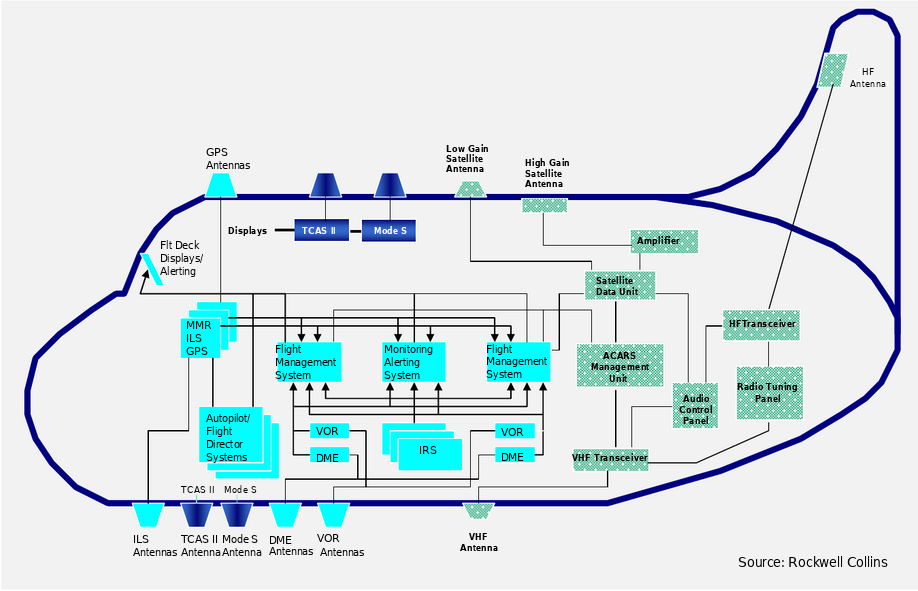
\includegraphics[scale=0.63]{images/current_avionics.png}
  \caption{Current avionics minimum requirements}
  \label{fig:modern}
\end{figure}

Although the OldGen provides some benefits in term of position accuracy and details for the controllers, there are still some problems:

- The information provided is still low and, except for the enhancements introduced with \textbf{Mode S}, it only provides a small aid during the flight.

- Using such protocols is still better than the radar alone; however, the accuracy level is still low and usually not much information can be carried so a intense verbal interaction with the controller is still required.

- There is no effective way to confirm the identity of an aircraft and the validity of the data that it is sending, thus allowing for no effort Man in the Middle and other attacks.

Different approaches to secure such protocols~\cite{nextgenenc} (both Old an NextGen) have been proposed. Unfortunately, none of them will be adopted in the transition to the NextGen but hopefully some may be used in the near future since there are studies and official documents about that~\cite{adsbimp}.

\bigskip

\section{NextGen and SESAR}

Both \textbf{NextGen} and \textbf{\acrshort{sesar}} (\acrlong{sesar}) are efforts to modernize the air transportation system respectively from the United States government and from the European Union along with other private parties. Both programs aim to achieve a higher degree of safety enhancing communications, navigation, surveillance technologies thus enabling all the users of the sky, even the future ones, to virtually see each other. The introduction of those new standards will also bring a reduction of costs through better \acrshort{atm} and enabling low visibility operations. The efforts are coordinated in order to assure a globally accepted common standard. For this reason from now on I will make no distinction and refer to both protocols as \textbf{NextGen}. However, many different protocols go under the \textbf{NextGen} family and some of them are not shared between Europe and America even if there are plans to do that.

The main component of this system is \acrlong{ads-b} (\textbf{\acrshort{ads-b}}).
\textit{"The American Federal Aviation Administration (FAA) as well as its European counterpart EUROCONTROL named ADS-B as the satellite-based successor of radar."}\cite{stroh14}
\textbf{\acrshort{ads-b}} is an automatic system which broadcasts aircraft sensors information to the outside world. It is divided in "ADS-B Out" which requires just a transponder able to properly encode messages and "ADS-B In" which requires a receiver, a computer and an interface to display the data.
\textbf{\acrshort{ads-b}} messages are also picked up by ground stations which feed the data to a central system where they are used, in combination with other data (e.g radars), to create a Traffic Situation Picture.

Two main protocols were proposed to deliver \textbf{\acrshort{ads-b}} messages:
\begin{itemize}
  \item \textbf{1090ES} (Extended Squitter)
  \item \textbf{\acrshort{uat}} (\acrlong{uat})
\end{itemize}

\textbf{1090ES} it is the current global standard for \textbf{\acrshort{ads-b}} in commercial aviation. In Europe \textbf{1090ES} is required for \acrshort{ifr} aircraft with a \acrshort{mtow} exceeding 12,566 pounds or maximum cruise airspeed faster than 250 KTAS. All aircrafts must comply with this regulation by 2020. \cite{eu1090}

In USA \textbf{1090ES} will be mandatory for all aircrafts after June 2020 and is the only technology that should be used when flying above 18,000 feet.
\cite{title14}. An overview of the USA supported technologies in the various airspace can be seen in Figure \ref{fig:uatvs1090}

This protocol is backward compatible with the \textbf{OldGen} since it uses the same frequencies and, in particular, a transponder supporting \textbf{Mode S} messages can be easily updated to support \textbf{\acrshort{ads-b}}. Therefore \textbf{\acrshort{ads-b}} information is simply carried inside a 112 bit \textbf{Mode S} message as it can be seen in Figure \ref{fig:1090es}. However, the message structure is different: The first 8 bits are used to identify the message and in particular the first 5 bits identify the type of message (10001 and 10010 for an \textbf{ADS-B} message) while the next 3 bits represent the capabilities which are different for every message type. The next 24 bits are the ICAO address of the aircraft. Then there are 56 bits containing data and the last 24 bits of \acrshort{crc} code. These last bits are particularly important as they allow to correct several errors in one message. All these characteristics are common with the \textbf{Mode S} messages so \textbf{ADS-B} messages encode their type and information in the 56 bits reserved to data. Data segments contains the first 5 bits indicating a type code for the \textbf{ADS-B} message and then other bits encode specific information depending on each message.\cite{modesbook}


\begin{figure}[htp]
\centering
\begin{minipage}{.5\textwidth}
  \centering
  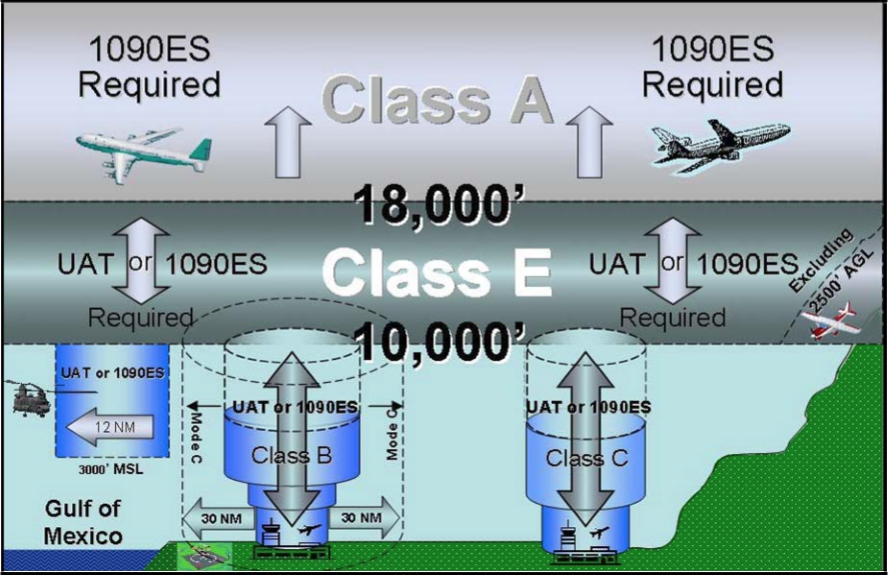
\includegraphics[scale=0.35]{images/uatvs1090.png}
  \caption{USA airspace}
  \label{fig:uatvs1090}
\end{minipage}%
\begin{minipage}{.5\textwidth}
  \centering
  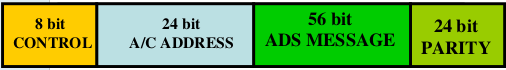
\includegraphics[scale=0.45]{images/1090es.png}
  \caption{1090ES Message}
  \label{fig:1090es}
\end{minipage}
\end{figure}

\textbf{\acrshort{uat}}-\acrlong{uat} is not actually Universal as it is not widespread yet like \textbf{1090ES}. This protocol is mainly deployed in North America and it is starting to be deployed also in China. It is not backward compatible with the \textbf{OldGen} and it was developed specifically to be used with \textbf{ADS-B}. It uses the 978MHz frequency and requires an entire new hardware to work.

However, since it is a newly designed protocol built to be future proof it allows to carry more information compared to \textbf{1090ES}, such as weather reports, pilots reports and other messages (like \acrshort{notam}s) using  \textbf{\acrshort{fis-b}} (\acrlong{fis-b}) and \textbf{\acrshort{tis-b}} (\acrlong{tis-b}), which are ground services that broadcast to "ADS-B In" equipped aircraft information on weather and traffic detected by ground radars as well as coming from other ADS-B equipped planes. Moreover \textbf{\acrshort{fis-b}} service is also capable to deliver real time weather images (\textbf{NexRad}) captured from the United States Weather Surveillance Radar through \textbf{ADS-B} messages. \textbf{NexRad} messages have the following format: \emph{<type> <hour>:<minute> <scale> <north> <west> <height> <width> <data>}

\emph{<type>} can be Regional (value 63) if the image represents a only a specific region of the map. Conus (value 64) if the image represents the whole (USA) map.

\emph{<scale>} can be 0, 1 or 2 and indicates the resolution of the image, an higher value means lower resolution.

\emph{<north> <west> <height> <width>} the first two elements refer to the respective edge of the block, their value is in arcminutes. The last two elements are the height and width of the block expressed in arcminutes of latitude and longitude.

The \emph{<data>} portion can be encoded in different ways:

- Run Length Encoding (RLE), particularly powerful as it has an high decompression speed.

- Empty Block representation, representing one or more block that are completly empty of data.

- Huffman Encoding, a common compression algorithm used in jpg images. It is based on a binary tree conveniently constructed using the occurrence of each character or element~\cite{huffman}.


US government is encouraging General Aviation (GA) aircrafts, not flying in Class A airspace, to use a \textbf{UAT} transponder. In this way there is less pollution of the 1090MHz frequency and they can receive more information such as weather data.

\textbf{Multilateration} is a technology which uses different signals to accurately locate an aircraft. It was initially developed for military purposes but was then adopted to confirm the position transmitted by \textbf{ADS-B}. It employs strategically placed antennas that listen to different replies (Mode A,C,S, military IFF and ADS-B) transmitted from an aircraft. Since a single aircraft will be at a different distance from every ground station, the replies to each station will have a different time of arrival; this difference can then be used to compute the precise position of an aircraft. This is the inverse of triangulation and requires no additional hardware since the ground stations are able to acquire replies from a multitude of different protocols. This also makes \textbf{multilateration} a faster method to locate an airplane since information can be acquired at a considerable higher rate. However, it has been demonstrated by Bran Haines in~\cite{haineshackfest} that such a system is not mandatory and rarely used.

\textbf{NextGen} protocols will also replace a big part of the voice communications not only between pilots and air traffic control but also between air traffic controllers themselves using the \textbf{\acrshort{uat}} data link and the previously mentioned \textbf{\acrshort{acars}} messages.
In particular \textbf{\acrshort{ads-c}} (\acrlong{ads-c}) automatically aggregate data such as aircraft position, altitude, speed, intent and meteorological data from on-board sensors. The generated report can then be sent to an ATS (\acrlong{ats}) unit or \acrshort{aoc} (\acrlong{aoc}) facility ground system for surveillance and route conformance monitoring \cite{goldman}. An \acrshort{ats} ground station must authenticate itself on the aircraft system to require a contract. Contracts can be of 3 types:

\begin{itemize}
  \item Periodic: the \acrshort{ats} specify the time interval at which the aircraft sends the report.
  \item Demand: a single report requested from the ground station. This request does not affect any other contracts that might be present.
  \item Emergency: these reports are tagged as "emergency" reports and will be highlighted to the \acrshort{atc}. Emergency reports can be generated manually by the crew or as a consequence of triggering another type of emergency system.
  \item Event: the \acrshort{ats} unit can specify the event (limited to 1 per aircraft) at which the report will be sent. The contract can contain multiple event types (e.g lateral deviation, vertical rate change ecc).
\end{itemize}

Security researchers in this field are focusing on \textbf{ADS-B} and various researches \cite{costin2012ghost,renderman} have already demonstrated the insecurity of such protocols in the \textbf{\acrshort{atc}/\acrshort{atm}} world. Few researches have been done on the aircraft side and it is now public and clear that this is a feasible entry point to an aircraft system~\cite{news-boeinghack-cso}.

\end{document}
